% Indicate the main file. Must go at the beginning of the file.
% !TEX root = ../main.tex

%----------------------------------------------------------------------------------------
% CHAPTER 4
%----------------------------------------------------------------------------------------
\chapter{Methodology} % Main chapter title
\label{Chapter4} % For referencing the chapter elsewhere, use \ref{Chapter1}

\section{Data}

The data was provided by [Eawag, institute of Aquatic Sciences]. It was generated using CADDIE2D software, which is described in Chapter \ref{Chapter3}. In the dataset, we look at four catchment areas around Switzerland, '26', '292', '709', '819' (see Fig \ref{fig:4.1}). They are named according to a DEM naming scheme all DEM's have a spatial resolution of 1. For each DEM, there are fourteen rainfall events (see \ref{fig:4.2}), for each rainfall event, there is a water depth  map for each time step (see Fig {fig:4.3}, which shows spatial evolution over time), rainfall event names, a mask to remove areas  outside the catchment area (if water were to propagate to this boundary, it would be considered run-off). Each time step represents 10 minutes of real time dynamics, but computational time of the CADDIES model varies.

\begin{figure}[htbp]
	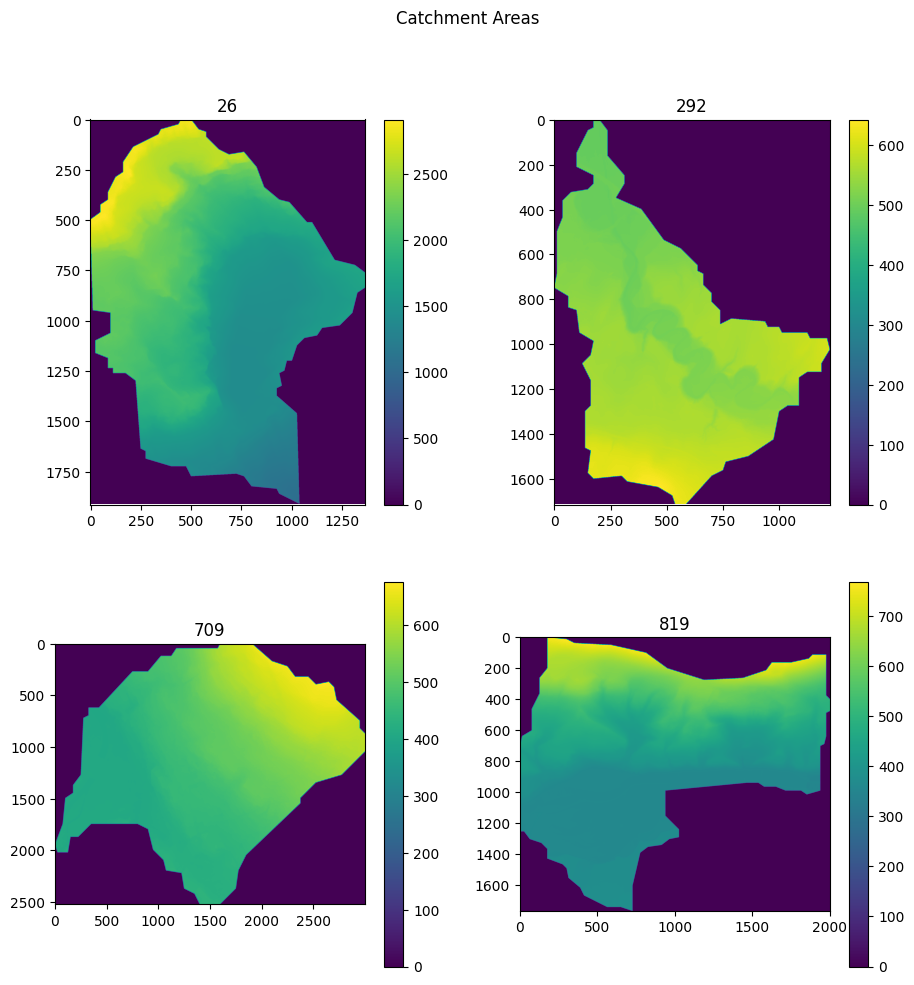
\includegraphics[width=0.6\textwidth]{../Figures/Catchment_dems.png}
	\centering
	\caption[FourDems]{Elevation map for the four catchment areas of interest. Color indicates height in m; height of 0 m is outside of the catchment area} 
	\label{fig:4.1}
\end{figure}

\begin{figure}[htbp]
	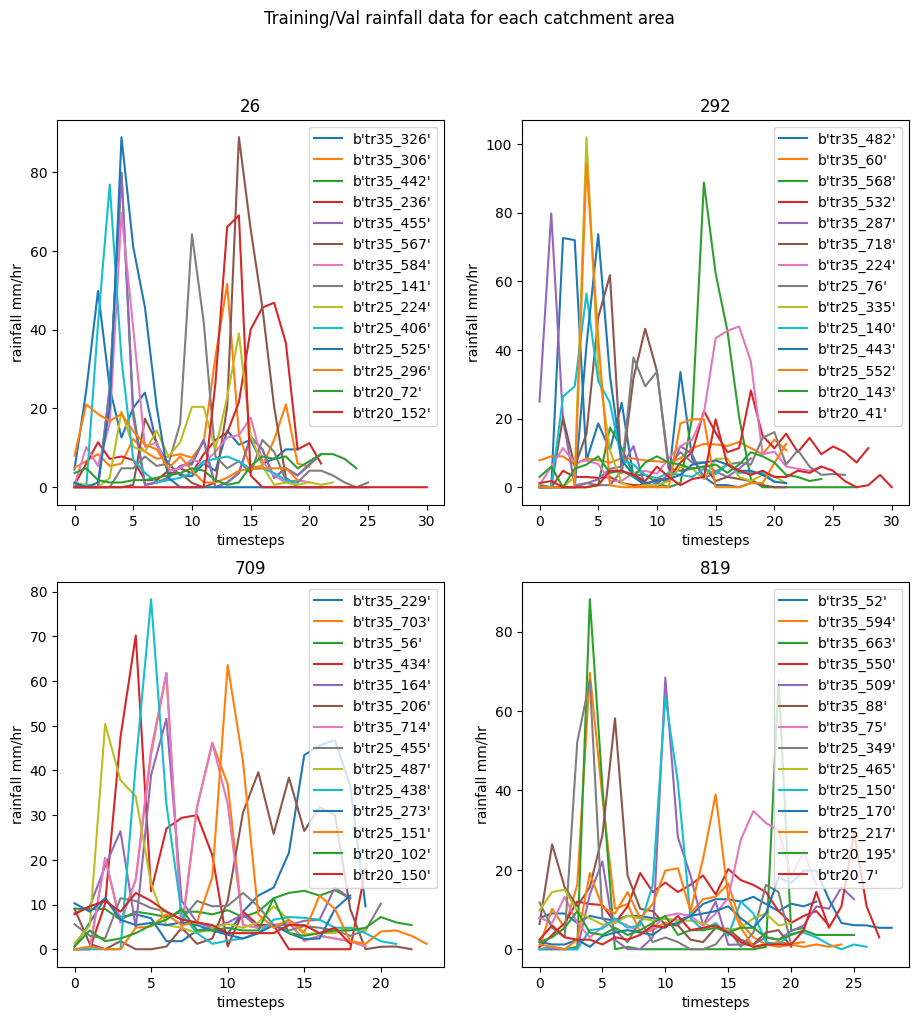
\includegraphics[width=0.6\textwidth]{../Figures/rainfall_train.png}
	\centering
	\caption[rainfall events]{Rainfall events over time for each DEM} 
	\label{fig:4.2}
\end{figure}

\begin{figure}[htbp]
	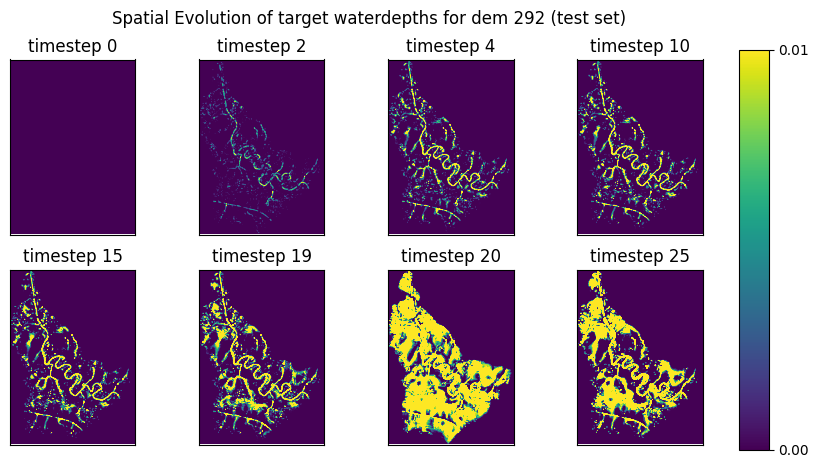
\includegraphics[width=0.6\textwidth]{../Figures/spatial_evoltution_waterdepth.png}
	\centering
	\caption[wd spatial evolution]{Spatial evolution of water depths for catchment 292. Colour indicates waterdepth (in m)} 
	\label{fig:4.3}
\end{figure}


\subsection{Data Preprocessing}
Due to computational limitations, data used during training are sub-sampled to have spatial dimensions 120 x 120, while the data used for testing has spatial dimensions 400 x 400 The rainfall events, titled "rainfall \_ events \_ 0 - 13", are used for training and validation data (using the train \_ test \_ split function from the sklearn library) in a ratio of 0.8 and 0.2 respectively. The last  rainfall  event "rainfall \_ events \_ 14" is unseen and used for the test set (see Fig \ref{fig:4.4}). \\
Many datasets were created but what has been mentioned above is consistent for all of them.

\begin{figure}[htbp]
	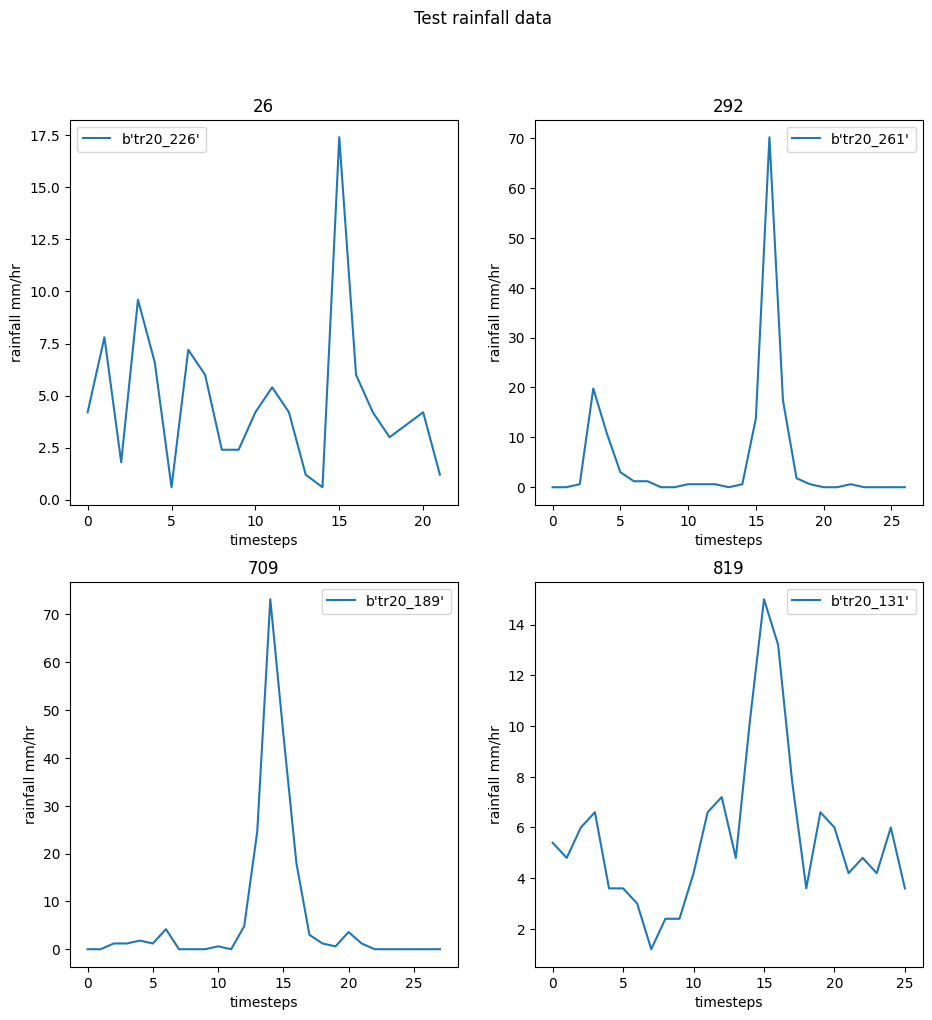
\includegraphics[width=0.6\textwidth]{../Figures/test_rainfall_events.png}
	\centering
	\caption[Rainfall Test]{Rainfall events used for testing} 
	\label{fig:4.4}
\end{figure}

\subsubsection*{Initial Screen}
Three datasets were created for each DEM. All datasets use the same features:
\begin{enumerate}
	\item Water depth (meters)
	\item Rainfall (mm/hr)
	\item DEM
\end{enumerate}

The first dataset uses the raw features generated by the CADDIES model. The second dataset uses Min Max normalization but across all features by normalizing via the DEM (see Eq. \ref{eq:4.1}). The third uses classical min max normalization (see Eq. \ref{eq:4.2}) for the DEM feature, rainfall is interpolated over time (see Eq \ref{eq:4.3})

\begin{equation}
	\label{eq:4.1}
	X_{norm} = \frac{X-A_{min}}{A_{max}-A_{min}}
\end{equation}

\begin{equation}
	\label{eq:4.2}
	X_{norm} = \frac{X-X_{min}}{X_{max}-X_{min}}
\end{equation}
Where $X$ is the feature to be normalized, $A$ is the whole dataset.
\begin{equation}
	\label{eq:4.3}
	r_{interpolated} = \frac{\frac{r}{1000}}{60} \times 10
\end{equation}
Where $r$ is rainfall in mm/hr. The interpolated rainfall is in m/ 10 minutes.

\subsubsection*{Initial Screen}



\section{Model creation}
\subsection{Classical CNN}
This was a baseline model. A generic approximation of grid search was done to find the optimial parameters.
\subsection{Gradient Filters}
A hardcoded kernel with sobel x, sobel y, and identity filters used as a way to to get gradients and information about the neighbourhood. which is then followed up with 1x1 convolutions for the computation. This filter comes straight from \cite{growing_nca}.

\subsection{Depthwise Convolusional Layer}
Instead of a 'hardcoded' filter to get gradients, the model learns should learn this filter for each feature and improves the models performance.


\subsection{NCA Model and Adaptions}
The model used is extremely similar to the model used in \cite{growing_nca} with some minor changes.

run an 80 filter, 3x3 kernel convolution over the input to create a feature map.

Then run 1x1 convolution, 128 layer deep, with activation relu.
pass that to another linear layer, output is the original channel count with no activation (although it might be possible to do something like sigmoid potentially due to the original caddieCA having a maximum allowed water transfer)

I make sure to not increment the DEM feature. I add alive masking (cell with \textless{} {0.01} m water depth is set to 0, because that's how the caddieCA model works (also something not done in the paper Joao sent us.))

The output of this model  becomes the new input, like a residual block.

\subsection{Loss}

\section{Evaluation}
\subsection{Custom L2 loss}
Due to the nature of the data (extremely small values), the loss starts off extrememly small (example of loss here based on real values). The model also really liked to predict 0 and try to just predict the last timestep. so we create a loss function to weight the 0's according to how many 0s appear in the data. We also try to mask it so that the model cannot predict less than 0 (constraint model)
\section{Proposed Evaluation}
The proposed evaluation of the model is based on a very simple heuristic. Can the model perform better than prediciting the previous timestep? (i.e. $\Delta{X_{t}} = \Delta{X_{t-1}}$)
\section{Pipeline Creation}
The creation of a pipline for training became extremely important for testing many parameters at once with different configurations for the dataset, training reigime, model creation. It allowed us to test multiple things in parrelel.